\documentclass[10pt,landscape,a4paper]{article}
\usepackage[utf8]{inputenc}
\usepackage[nosf]{kpfonts}
\usepackage[t1]{sourcesanspro}

% For the multiple columns in the cheat sheet
\usepackage{multicol}

% Set the margins of the paper
\usepackage[margin=1mm]{geometry}

% To use colours
\usepackage{xcolor}

% To typeset small fonts
\usepackage{microtype}

% To have easier typesetting of units
\usepackage{siunitx}

% To draw arrows in a table
\usepackage{tikz}
\usetikzlibrary{tikzmark}

% To include graphics
\usepackage{graphicx}

\graphicspath{ {./images/} }

\let\bar\overline

\definecolor{myblue}{cmyk}{1,.72,0,.38}

\everymath\expandafter{\the\everymath \color{myblue}}
\everydisplay\expandafter{\the\everydisplay \color{myblue}}

\renewcommand{\baselinestretch}{.8}
\pagestyle{empty}

\makeatletter
\renewcommand{\section}{\@startsection{section}{1}{0mm}%
  {.2ex}%
  {.2ex}%x
  {\color{myblue}\sffamily\small\bfseries}}
\renewcommand{\subsection}{\@startsection{subsection}{1}{0mm}%
  {.2ex}%
  {.2ex}%x
  {\sffamily\bfseries}}
\renewcommand{\subsubsection}{\@startsection{subsubsection}{1}{0mm}%
  {.2ex}%
  {.2ex}%x
  {\sffamily\bfseries}}


\makeatother
\setlength{\parindent}{0pt}

\begin{document}
\small
\begin{multicols*}{5}
  \raggedcolumns

  \section{Definitions}
  \(\Diamond\) Differentiator: \(ks, \text{ where } k \text{ is a constant}\) \\
  \(\Diamond\) Integrator: \(\frac{k}{s}, \text{ where } k \text{ is a constant}\) \\
  \(\Diamond\) Dominant poles are the \textbf{rightmost} poles.


  \section{Transfer function}
  Feedback path transfer function: \(H(s)\)

  Negative or unity (\(H(s) = 1\)) feedback: \\
  \(CLTF = \frac{\text{Forward path TF}}{1 + H(s) (\text{Forward path TF})}\)

  Positive feedback: \\
  \(CLTF = \frac{\text{Forward path TF}}{1 - H(s) (\text{Forward path TF})}\)


  \section{Mason's gain formula}
  Formula: \(\frac{C(s)}{R(s)} = \sum_{k = 1}^n \frac{T_k \Delta_k}{\Delta}\)

  \(T_k\): Gain of the \(k^{th}\) \textbf{forward path}.

  Determinant (\(\Delta\)): \\
  \(\Diamond\) Sum the gain for all individual loops. \\
  \(\Diamond\) Sum the gain products for 2 non-touching loops, then 3, then 4, and so on, \textbf{adding} the \textbf{even-numbered} gain products and subtracting the \textbf{odd-numbered} gain products. \\
  \(\Delta = 1 - \text{Sum of the previous 2 steps}\)

  Associated path factor (\(\Delta_k\)): \\
  \(\Diamond\) The part of \(\Delta\) \textbf{not touching} the \(k^{th}\) forward path.

  \subsection{Steps}
  \(\Diamond\) Get the gains for all \textbf{forward paths}. \\
  \(\Diamond\) Get the gains for all \textbf{loops}. \\
  \(\Diamond\) Get the gains for all \textbf{non-touching loops}, then use the formula to solve.


  \section{Mathematical modelling}
  Newton's 2nd law: \(F = ma = I \alpha\) \\
  Torque: \(T = Fd_{\perp}\) \\
  Spring: \(\mathcal{L} \left\{kx \right\} = KX(s)\) \\
  Damper: \(\mathcal{L} \left\{cv \right\} = \mathcal{L} \left\{c \dot{x} \right\} = cs X(s)\)

  Mass acceleration due to gravity: \\
  \(\mathcal{L} \left\{Ma \right\} = \mathcal{L} \left\{M \ddot{x} \right\} = Ms^2 X(s)\)

  Moment of inertia: \\
  \(\mathcal{L} \left\{I \alpha \right\} = \mathcal{L} \left\{I \ddot{\theta} \right\} = Is^2 \Theta (s)\)

  Gear ratio (direction is important): \\
  \(n = \frac{\text{Driving}_1}{\text{Driven}_2} = \frac{r_1}{r_2} = \frac{N_1}{N_2} = \frac{T_1}{T_2} = \frac{\omega_2}{\omega_1} = \frac{\theta_2}{\theta_1}\)

  Gear ratio for inertia and damping: \(n^2\)


  \section{Poles and stability}

  Characteristic equation of \(G(s) = \frac{N(s)}{D(s)}\): \\
  \(\text{Denominator: } D(s) = 0\)

  \(\Diamond\) Transfer function poles are the \textbf{roots of the characteristic equation}.

  \subsection{BIBO stability}
  \(\Diamond\) A system is bounded-input bounded-output (BIBO) stable if the output is bounded when the input is bounded. \\
  \(\Diamond\) \textbf{Stable systems} have poles with \textbf{negative real parts}, like \(-1\) or \(-1 + j\). \\
  \(\Diamond\) \textbf{Partially-stable systems} have \textbf{imaginary poles}, like \(- j\) or \(- 2j\). \\
  \(\Diamond\) \textbf{Unstable systems} have poles with \textbf{positive real parts}, like \(1\) or \(1 - 2j\).

  \subsection{Routh-Hurwitz criterion}
  \(\Diamond\) If there are \textbf{no sign changes} in the first column, the system is \textbf{stable}. \\
  \(\Diamond\) If one of the elements in the first column is 0, replace the zero with \(\varepsilon\), which is a small positive number. The system is \textbf{partially stable} if there are \textbf{no sign changes}, and \textbf{partially unstable} if there are \textbf{sign changes} in the first column. \\
  \(\Diamond\) If an entire row of elements are 0, form an equation with the row \(s\) above it and \textbf{differentiate} the equation with respect to \(s\). The system is \textbf{partially stable} if there are \textbf{no sign changes}, and \textbf{partially unstable} if there are \textbf{sign changes} in the first column.

  \subsubsection{Method}
  For the characteristic equation: \\
  \(s^4 + 5s^3 + 10s^2 + 50s + 100 = 0\)

  \begin{tabular}{@{}c|ccc}
    \hline
    \(s^4\) & \(1\)\tikzmark{1a} & \tikzmark{10a}\(10\) & \(100\) \\
    \(s^3\) & \(5\)\tikzmark{5a} & \tikzmark{50a}\(50\) & \(0\) \\
    \(s^2\) & \(\frac{5 \times 10 - 1 \times 50}{5}\) \\
    \(s^1\) \\
    \(s^0\) \\
  \end{tabular}

  \begin{tikzpicture}[overlay, remember picture, transform canvas={yshift=.25\baselineskip}]
    \draw [->, green] ([xshift=1pt]{pic cs:5a}) -- node[above, green, near end]{+} ({pic cs:10a});
    \draw [->, red] ({pic cs:1a}) -- node[below, red, near end]{-} ({pic cs:50a});
  \end{tikzpicture}

  \begin{tabular}{@{}c|ccc}
    \hline
    \(s^4\) & \(1\)\tikzmark{1b} & \(10\) & \tikzmark{100b}\(100\) \\
    \(s^3\) & \(5\)\tikzmark{5b} & \(50\) & \tikzmark{0b}\(0\) \\
    \(s^2\) & \(0\) & \(\frac{5 \times 100 - 1 \times 0}{5}\) \\
    \(s^1\) \\
    \(s^0\) \\
  \end{tabular}

  \begin{tikzpicture}[overlay, remember picture, transform canvas={yshift=.25\baselineskip}]
    \draw [->, green] ([xshift=1pt]{pic cs:5b}) -- node[above, green, near end]{+} ([yshift=-1pt]{pic cs:100b});
    \draw [->, red] ([yshift=1pt]{pic cs:1b}) -- node[below, red, near end]{-} ([yshift=1pt]{pic cs:0b});
  \end{tikzpicture}

  \begin{tabular}{@{}c|ccc}
    \hline
    \(s^4\) & \(1\) & \(10\) & \(100\) \\
    \(s^3\) & \(5\)\tikzmark{5c} & \tikzmark{50c}\(50\) & \(0\) \\
    \(s^2\) & \(\varepsilon\)\tikzmark{ec} & \tikzmark{100c}\(100\) \\
    \(s^1\) & \(\frac{50 \times \varepsilon - 5 \times 100}{\varepsilon}\) & \(0\) \\
    \(s^0\) \\
  \end{tabular}

  \begin{tikzpicture}[overlay, remember picture, transform canvas={yshift=.25\baselineskip}]
    \draw [->, green] ({pic cs:ec}) -- node[above, green, near end]{+} ({pic cs:50c});
    \draw [->, red] ([xshift=1pt]{pic cs:5c}) -- node[below, red, near end]{-} ({pic cs:100c});
  \end{tikzpicture}

  \begin{tabular}{@{}c|ccc}
    \hline
    \(s^4\) & \(1\) & \(10\) & \(100\) \\
    \(s^3\) & \(5\) & \(50\) & \(0\) \\
    \(s^2\) & \(\varepsilon\)\tikzmark{ed} & \tikzmark{100d}\(100\) \\
    \(s^1\) & \(\frac{50 \varepsilon - 500}{\varepsilon}\)\tikzmark{fracd} & \tikzmark{0d}\(0\) \\
    \(s^0\) & \(\frac{50 \varepsilon - 500}{\varepsilon}\) \\
  \end{tabular}

  \begin{tikzpicture}[overlay, remember picture, transform canvas={yshift=.25\baselineskip}]
    \draw [->, green] ({pic cs:fracd}) -- node[above, green, midway]{+} ({pic cs:100d});
    \draw [->, red] ([xshift=1pt]{pic cs:ed}) -- node[below, red, near end]{-} ({pic cs:0d});
  \end{tikzpicture}

  Since \(\varepsilon\) is a small positive number, let \(\varepsilon = 1\).

  \begin{tabular}{@{}c|ccc}
    \hline
    \(s^4\) & \(1\) & \(10\) & \(100\) \\
    \(s^3\) & \(5\) & \(50\) & \(0\) \\
    \(s^2\) & \(\varepsilon\) & \(100\) \\
    \(s^1\) & \(\frac{50(1) - 500}{1} = -450\) & \(0\) \\
    \(s^0\) & \(\frac{50(1) - 500}{1} = -450\) \\
  \end{tabular}

  Since there is a sign change in the first column, the system is \textbf{partially unstable}.

  \vspace{20em}


  \section{Second order system response}
  Impulse input: \(R(s) = A\) \\
  Step input: \(R(s) = \frac{A}{s}\) \\
  Ramp input: \(R(s) = \frac{A}{s^2}\) \\
  Sinusoidal input: \(R(s) = \frac{\omega}{s^2 + \omega^2}\)

  General formula: \\
  \(G(s) = \frac{\omega_n^2}{s^2 + 2 \zeta \omega_n s + \omega_n^2}\)

  Undamped or natural frequency: \(\omega_n\)

  Damping ratio (\(\zeta\)): \\
  \(0 < \zeta_{under} < 1, \quad \zeta_{crit} = 1, \quad \zeta_{over} > 1\)

  Damped natural frequency: \\
  \(\omega_d = \omega_n \sqrt{1 - \zeta^2}\)

  Angle: \\
 \(\phi = \arctan \frac{\omega_d}{\zeta \omega_n}\)

  Rise time: \\
  \(t_r = \frac{\pi - \phi}{\omega_d}\)

  Peak time: \\
  \(t_p = \frac{\pi}{\omega_d}\)

  Maximum overshoot: \\
  \(M_p = e^{- \frac{\zeta \pi}{\sqrt{1 - \zeta^2}}} \times 100 \%\)

  Settling time: \\
  \(t_s = 3T = \frac{3}{\zeta \omega_n}\) for 5\% criterion \\
  \(t_s = 4T = \frac{4}{\zeta \omega_n}\) for 2\% criterion


  \section{Steady state analysis}
  DC gain, or response to unit step input: \\
  \(\lim_{s \rightarrow 0} s G(s) \left(\frac{1}{s} \right) = \lim_{s \rightarrow 0} G(s)\)

  Position error constant (\(k_{pos}\)): \\
  \(k_{pos} = \lim_{s \rightarrow 0} G(s)\) \\
  \(e(\infty) = \frac{1}{1 + k_{pos}}\)

  Velocity error constant (\(k_{vel}\)): \\
  \(k_{vel} = \lim_{s \rightarrow 0} s G(s)\) \\
  \(e(\infty) = \frac{1}{k_{vel}}\)

  Acceleration error constant (\(k_{acc}\)): \\
  \(k_{acc} = \lim_{s \rightarrow 0} s^2 G(s)\) \\
  \(e(\infty) = \frac{1}{k_{acc}}\)

  \section{Root locus}

  Open-loop poles: \(p\) \\
  Open-loop zeros: \(z\)

  Characteristic equation: \\
  \(1 + K \frac{N(s)}{D(s)} = 0, \text{ where } K \frac{N(s)}{D(s)} \text{ is the OLTF}\)

  Starting points: \\
  \(\text{Denominator: } D(s) = 0\)

  Ending points: \\
  \(\text{Numerator: } N(s) = 0\)

  Asymptote angle, open-loop zeros at \(\infty\): \\
  \(\angle s = \frac{\pi (1 + 2q)}{N_{poles} - N_{zeros}}, \text{ where } q = 0, 1, 2, \ldots\)

  Asymptote location: \\
  \(\sigma_a = \frac{\sum(\mathrm{Re}(p)) - \sum (\mathrm{Re}(z))}{N_{poles} - N_{zeros}}\)

  Break-in or break-out points: \\
  \(\frac{dK}{ds} = 0, \text{ reject points not on the locus}\)

  Phase condition: \\
  \(\sum \angle (s + z) - \sum \angle (s + p) = \pm \pi\)

  \subsection{Departure and arrival angles}
  \(\Diamond\) Take a point infinitesimally close to one of the \textbf{starting points} or \textbf{poles} for the \textbf{departure angle}, or one of the \textbf{ending points} or \textbf{zeros} for the \textbf{arrival angle}. \\
  \(\Diamond\) Calculate the angles to the point for each pole and zero and use the phase condition above to find the remaining angle. \\
  \(\Diamond\) The angle for the lines must \textbf{start} from the \textbf{right side} of the point, rotating \textbf{anti-clockwise}.

  \subsection{Intersection of the imaginary axis}
  Substitute \(s = j \omega\) into the characteristic equation and solve for \(K\) and \(\omega\).

  \subsection{Drawing the root locus}
  \(\Diamond\) Number all the points on the \textbf{real-axis}, starting from 1, and from the \textbf{right side} going to the \textbf{left}.
  \(\Diamond\) Every \textbf{odd-numbered} point on the \textbf{real axis}, regardless of whether it is a zero or a pole, has a root locus to the \textbf{left} of it.

  \section{Controllers}

  PD controller: \\
  \(G_c (s) = K_P + K_D s = K_D (s + z_c)\)

  PI controller: \\
  \(G_c (s) = K_P + \frac{K_I}{s} = \frac{K_P (s + z_c)}{s}\) \\
  \(\Diamond\) When \(z_c\) is small (\(0 < z_c < 1\)), pole-zero cancellation occurs and the transient response is only slightly affected.

  Phase (lead or lag) compensator: \\
  \(G_c (s) = K \frac{s + z}{s + p}\)

  PID controller: \\
  \(G_c (s) = K_P + K_D s + \frac{K_I}{s}\) \\
  \(\Diamond\) PD to tune transient response. \\
  \(\Diamond\) PI to eliminate steady-state error.

  Lead-lag compensator: \\
  \(G_c (s) = K_1 \frac{s + z_1}{s + p_1} + K_2 \frac{s + z_2}{s + p_2}\) \\
  \(\Diamond\) Lead compensator to tune transient response. \\
  \(\Diamond\) Lag compensator to reduce steady-state error.

  \subsection{Designing controllers}
  \(\Diamond\) Form equation in \(s\) using desired roots. \\
  \(\Diamond\) Use arbitrary roots if there are higher powers of \(s\) in the transfer function. \\
  \(\Diamond\) Equate the denominator of the closed-loop transfer function with the controller to the equation with the desired roots and solve for the unknowns.

  \section{Bode plots}
  \(\Diamond\) Break down complex functions into \textbf{individual functions} and graph the asymptotes individually before adding them to get the net asymptote. \\
  \(\Diamond\) Magnitudes must always be in decibels, i.e. \(20 \lg \omega\). \\
  \(\Diamond\) Corner frequencies are always \(0.1a, a\), and \(10a\). \\
  \(\Diamond\) Must always show peaks if the damping ratio (\(\zeta\)) is less than \(\frac{1}{\sqrt{2}}\).

  \subsection{Graphs}

  Constants \(\left(G(s) = K \right)\): \\
  \(G(s = j \omega) = Ke^{j0}\) \\
  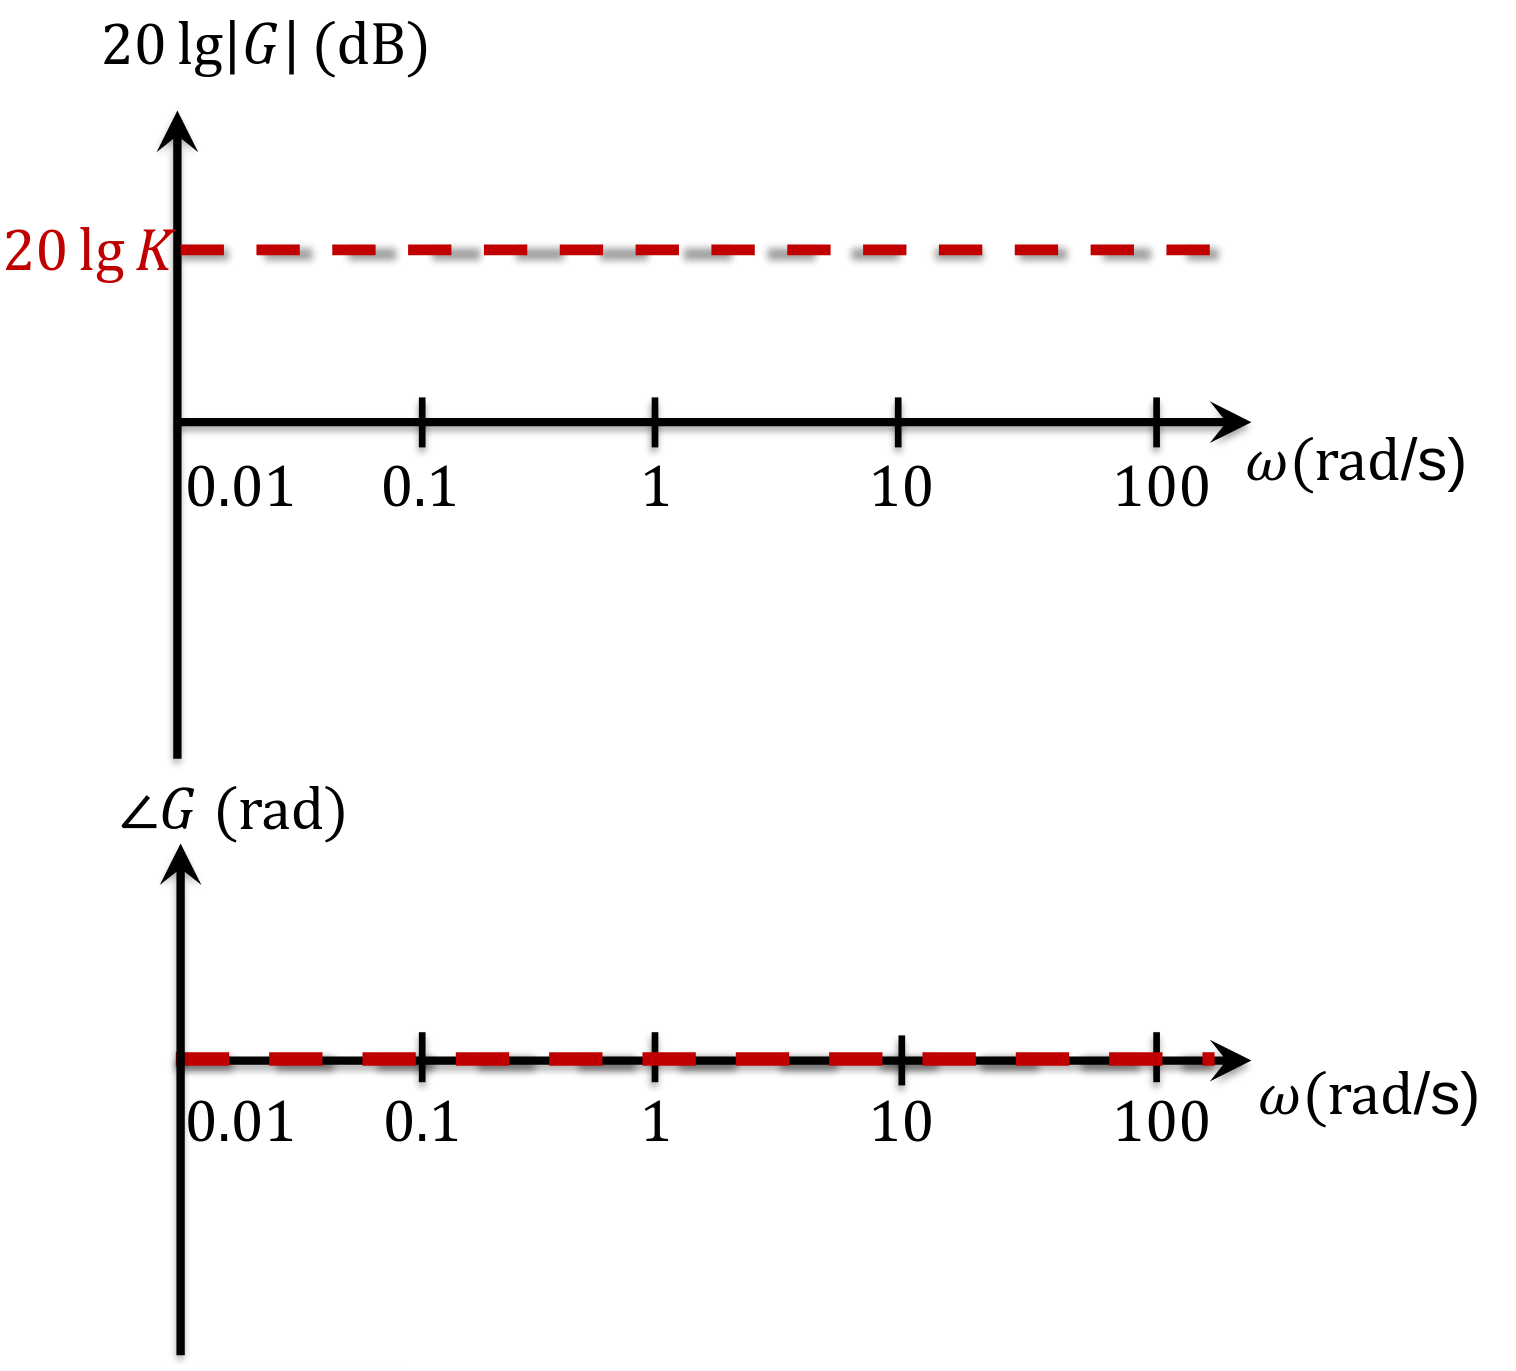
\includegraphics[width=\linewidth]{bode-plots-constant-plots.png}

  Differentiator \(\left(G(s) = s \right)\): \\
  \(G(s = j \omega) = \omega e^{j \frac{\pi}{2}}\) \\
  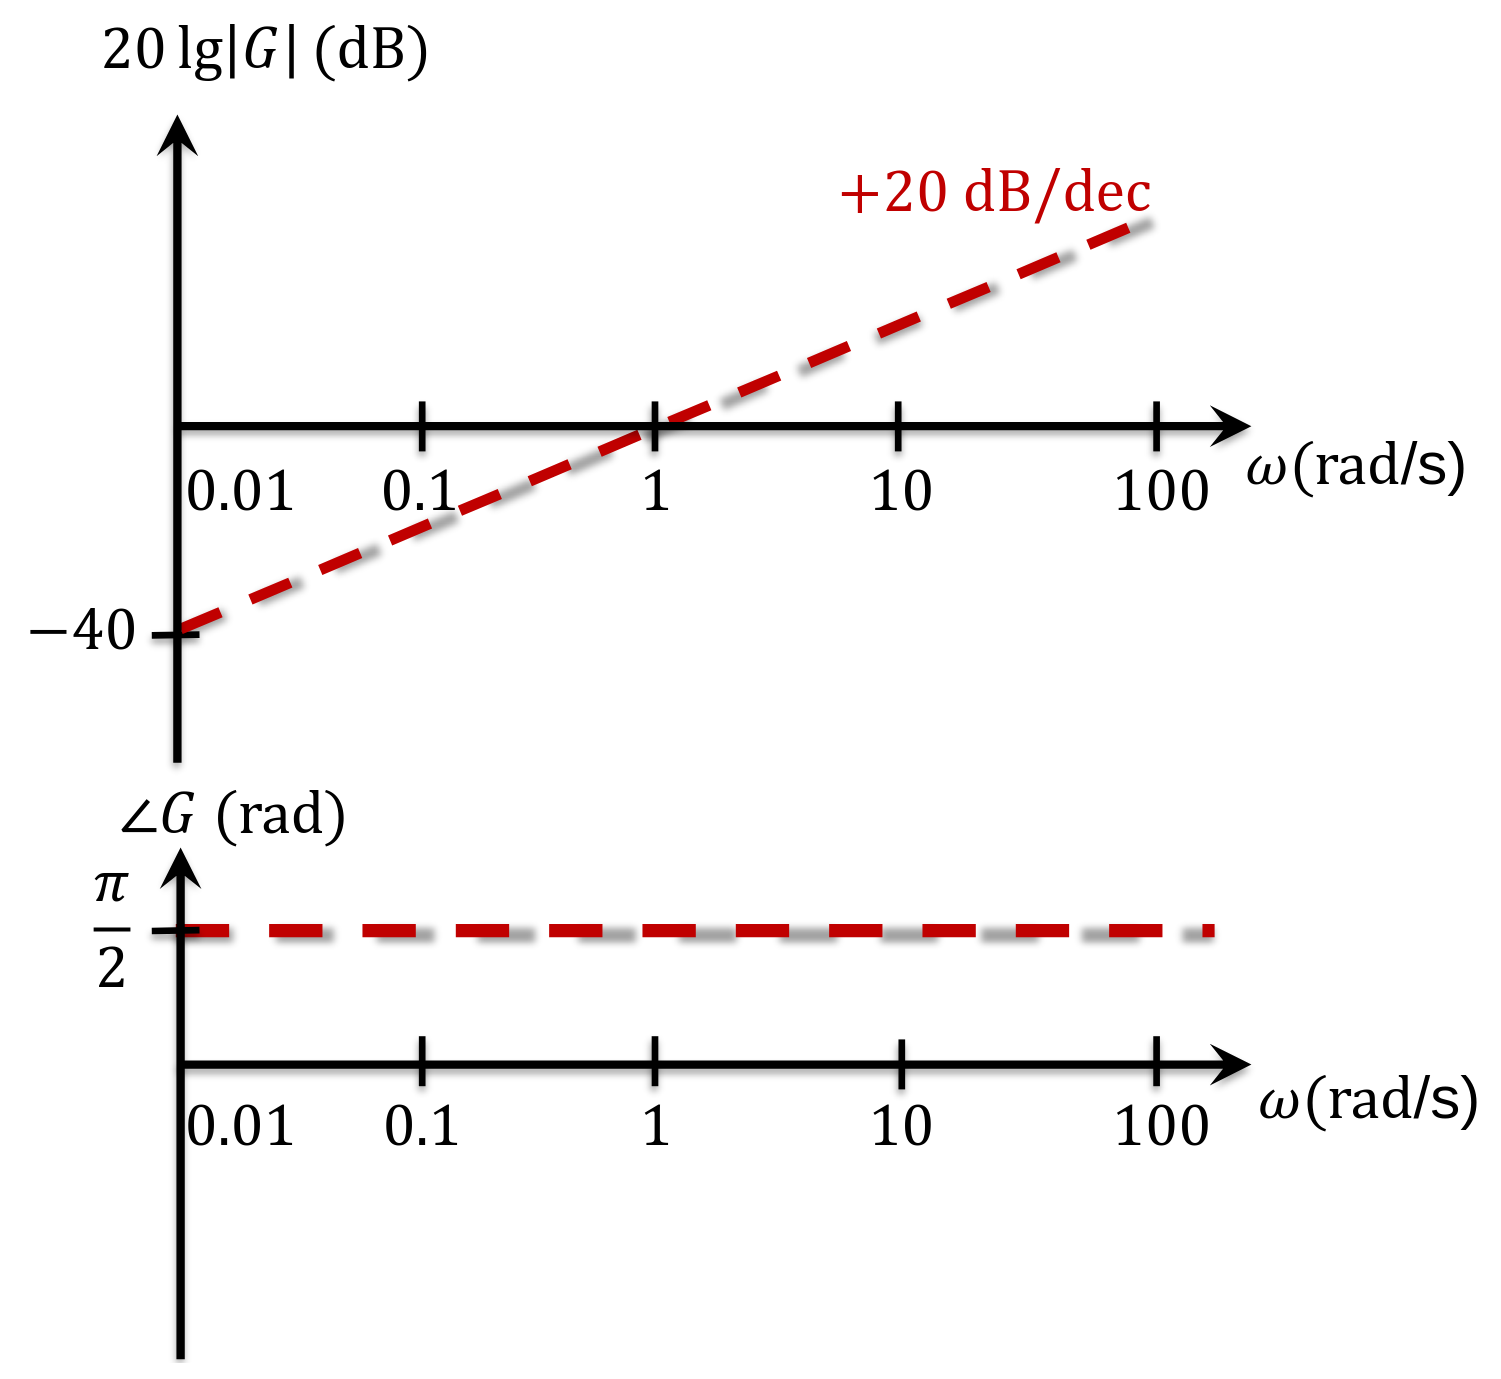
\includegraphics[width=\linewidth]{bode-plots-differentiator-plots.png}

  Integrator \(\left(G(s) = \frac{1}{s} \right)\): \\
  \(G(s = j \omega) = \frac{1}{\omega} e^{j \left(-\frac{\pi}{2} \right)}\) \\
  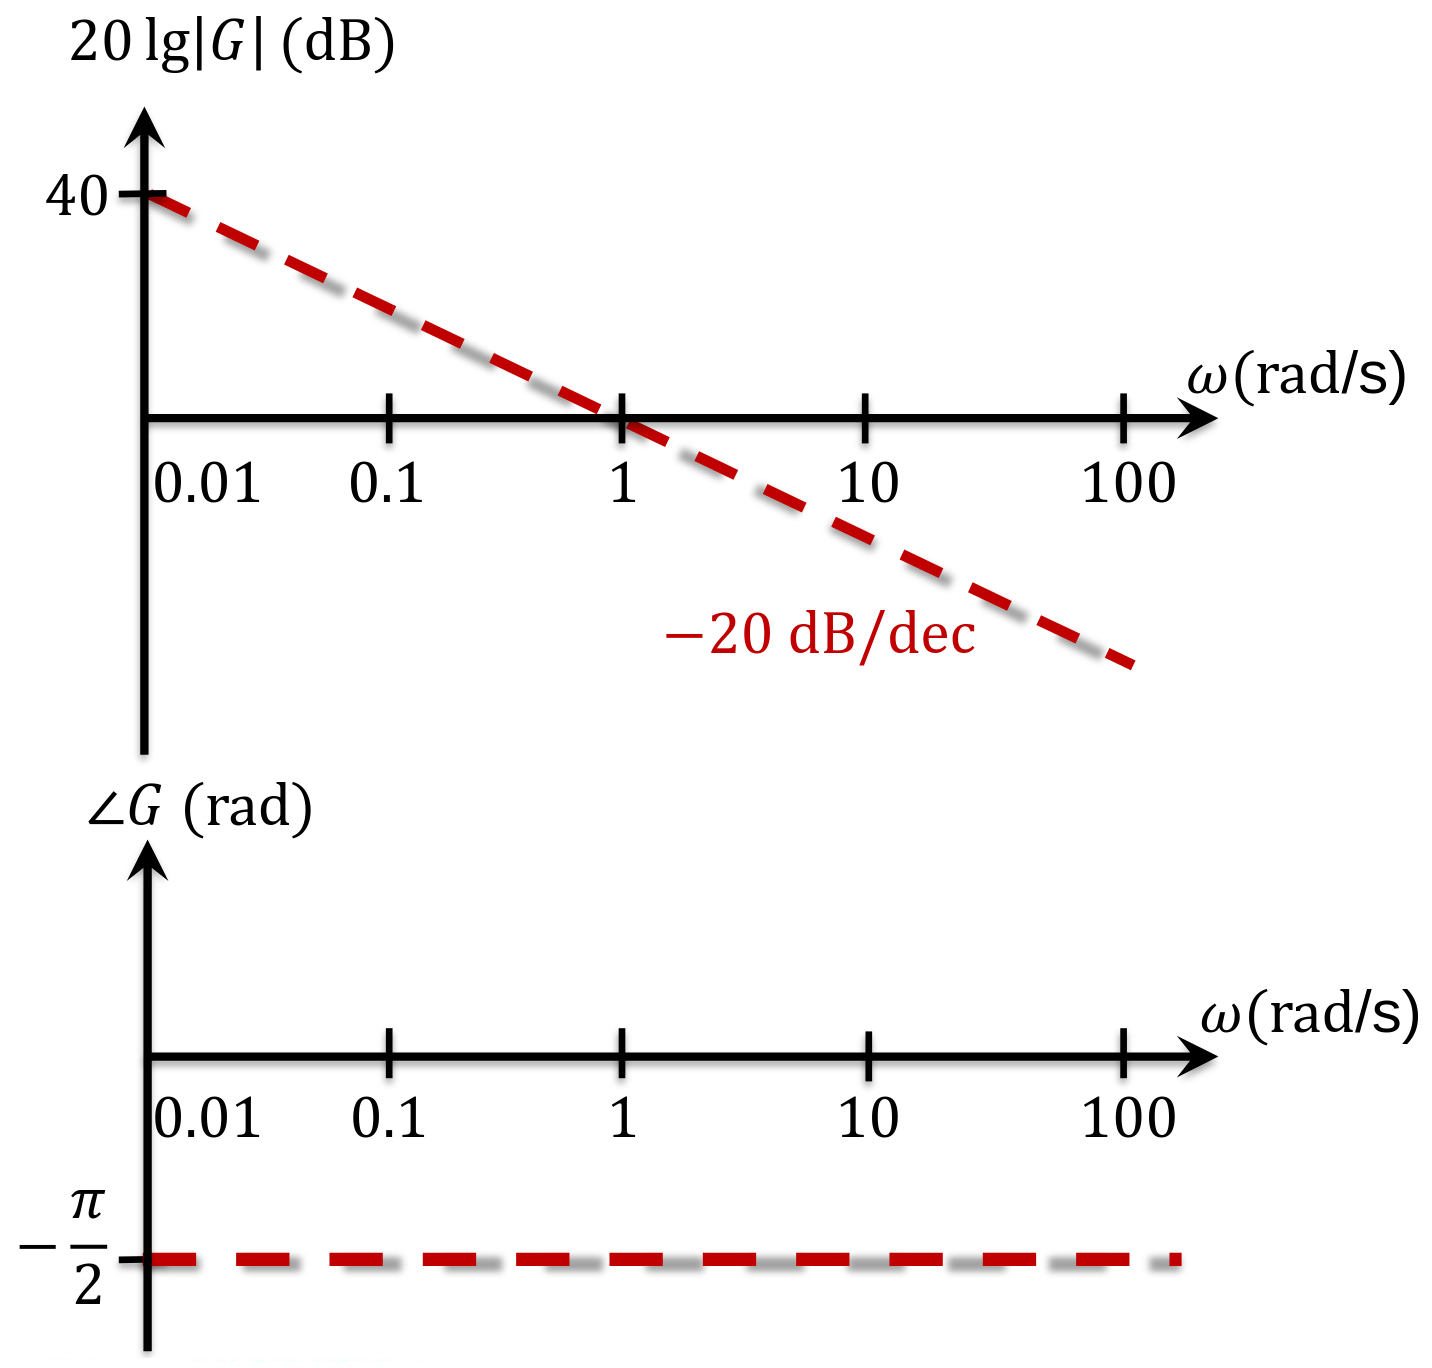
\includegraphics[width=\linewidth]{bode-plots-integrator-plots.png}

  \vspace{1em}

  First order pole \(\left(G(s) = \frac{a}{s + a} \right)\): \\
  When \(\omega << a\): \(G(s = j \omega) = 1e^{j0}\) \\
  When \(\omega >> a\): \(G(s = j \omega) = \frac{a}{\omega} e^{j \left(-\frac{\pi}{2} \right)}\) \\
  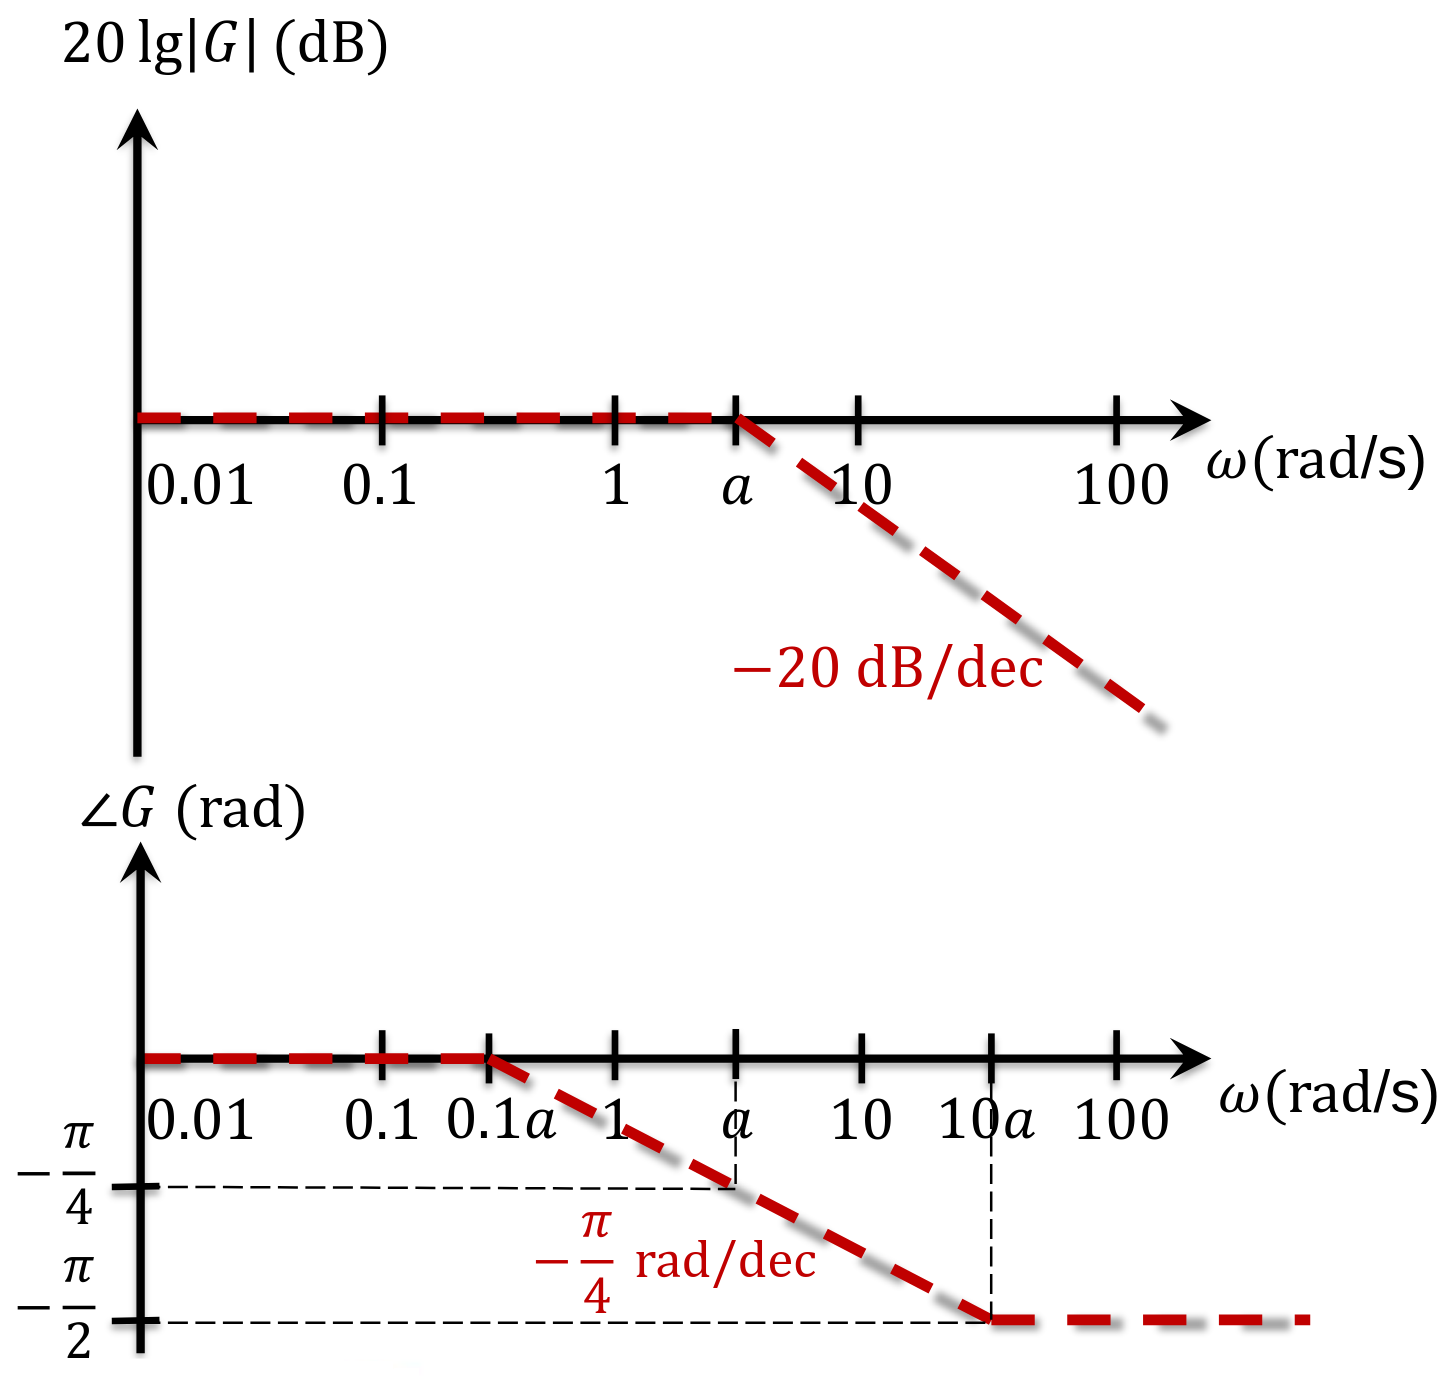
\includegraphics[width=\linewidth]{bode-plots-first-order-pole-plots-2.png}

  First order zero \(\left(G(s) = \frac{s + a}{a} \right)\): \\
  When \(\omega << a\): \(G(s = j \omega) = 1e^{j0}\) \\
  When \(\omega >> a\): \(G(s = j \omega) = \frac{\omega}{a} e^{j \frac{\pi}{2}}\) \\
  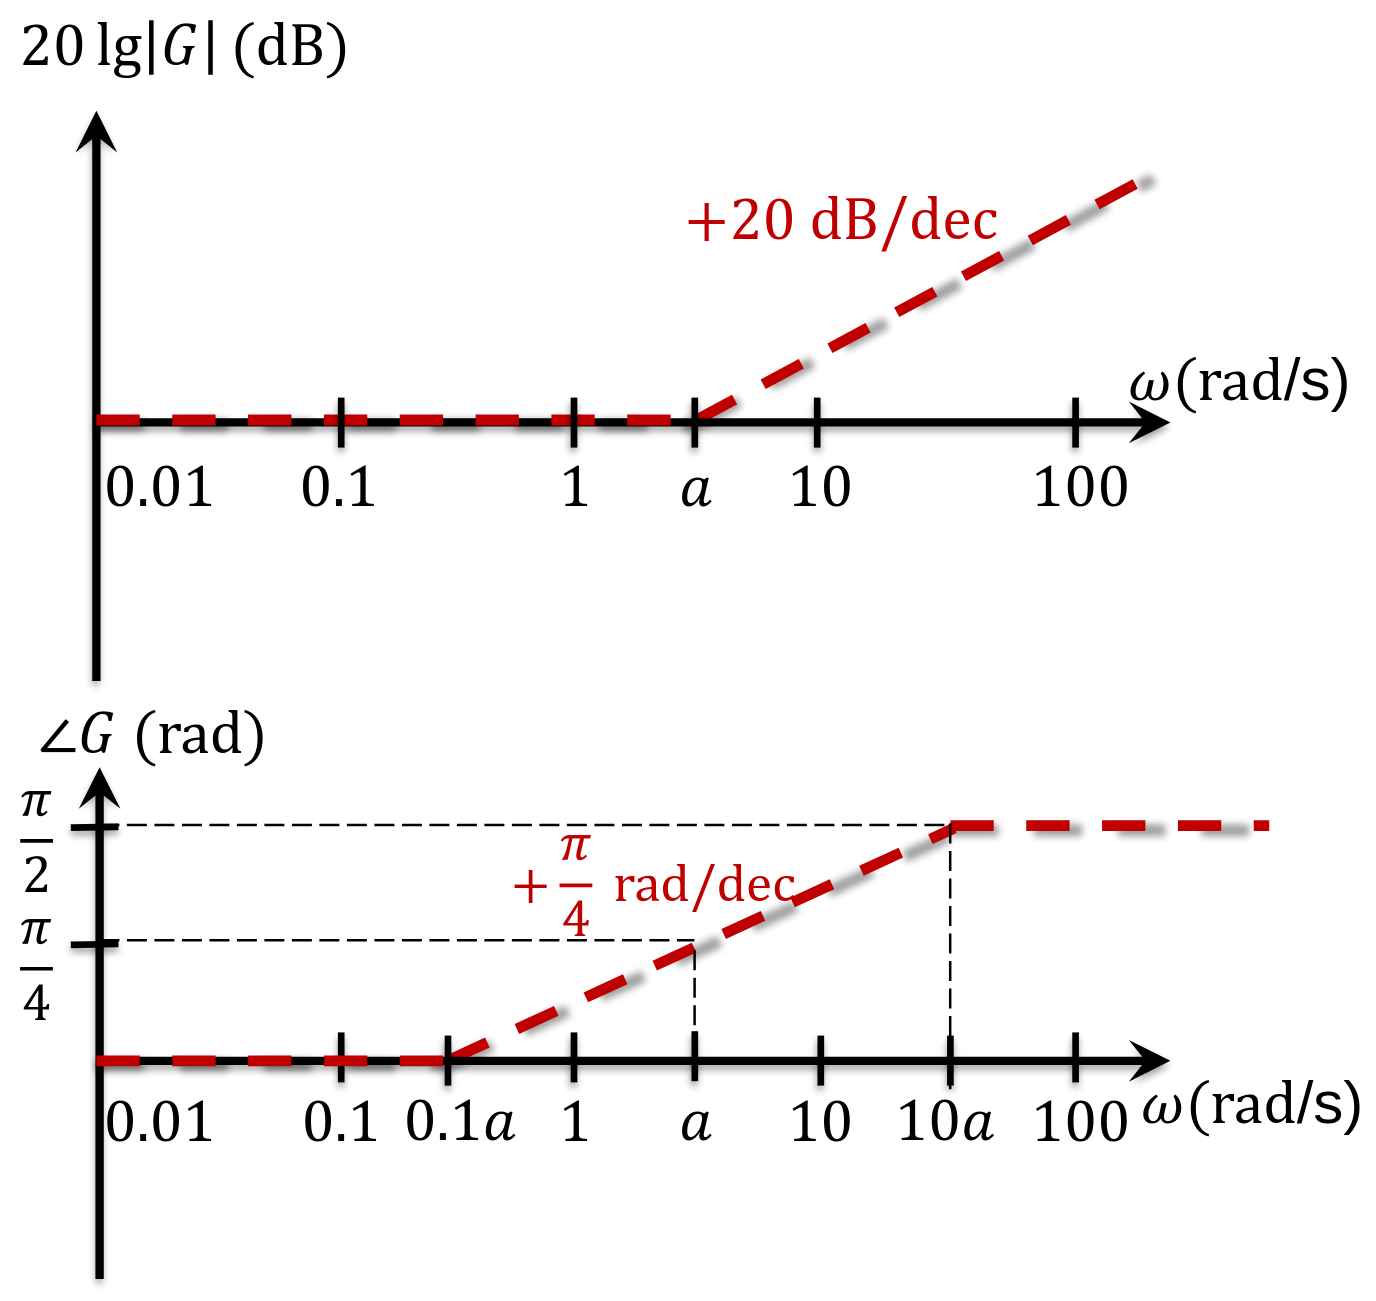
\includegraphics[width=\linewidth]{bode-plots-first-order-zero-plots-2.png}

  Second order pole \(\left(G(s) = \frac{\omega_n^2}{s^2 + 2 \zeta_n s + \omega_n^2} \right)\): \\
  When \(\omega << \omega_n\): \(G(s = j \omega) = 1e^{j0}\) \\
  When \(\omega >> \omega_n\): \(G(s = j \omega) = \frac{\omega_n^2}{\omega^2} e^{j \left(-\pi \right)}\) \\
  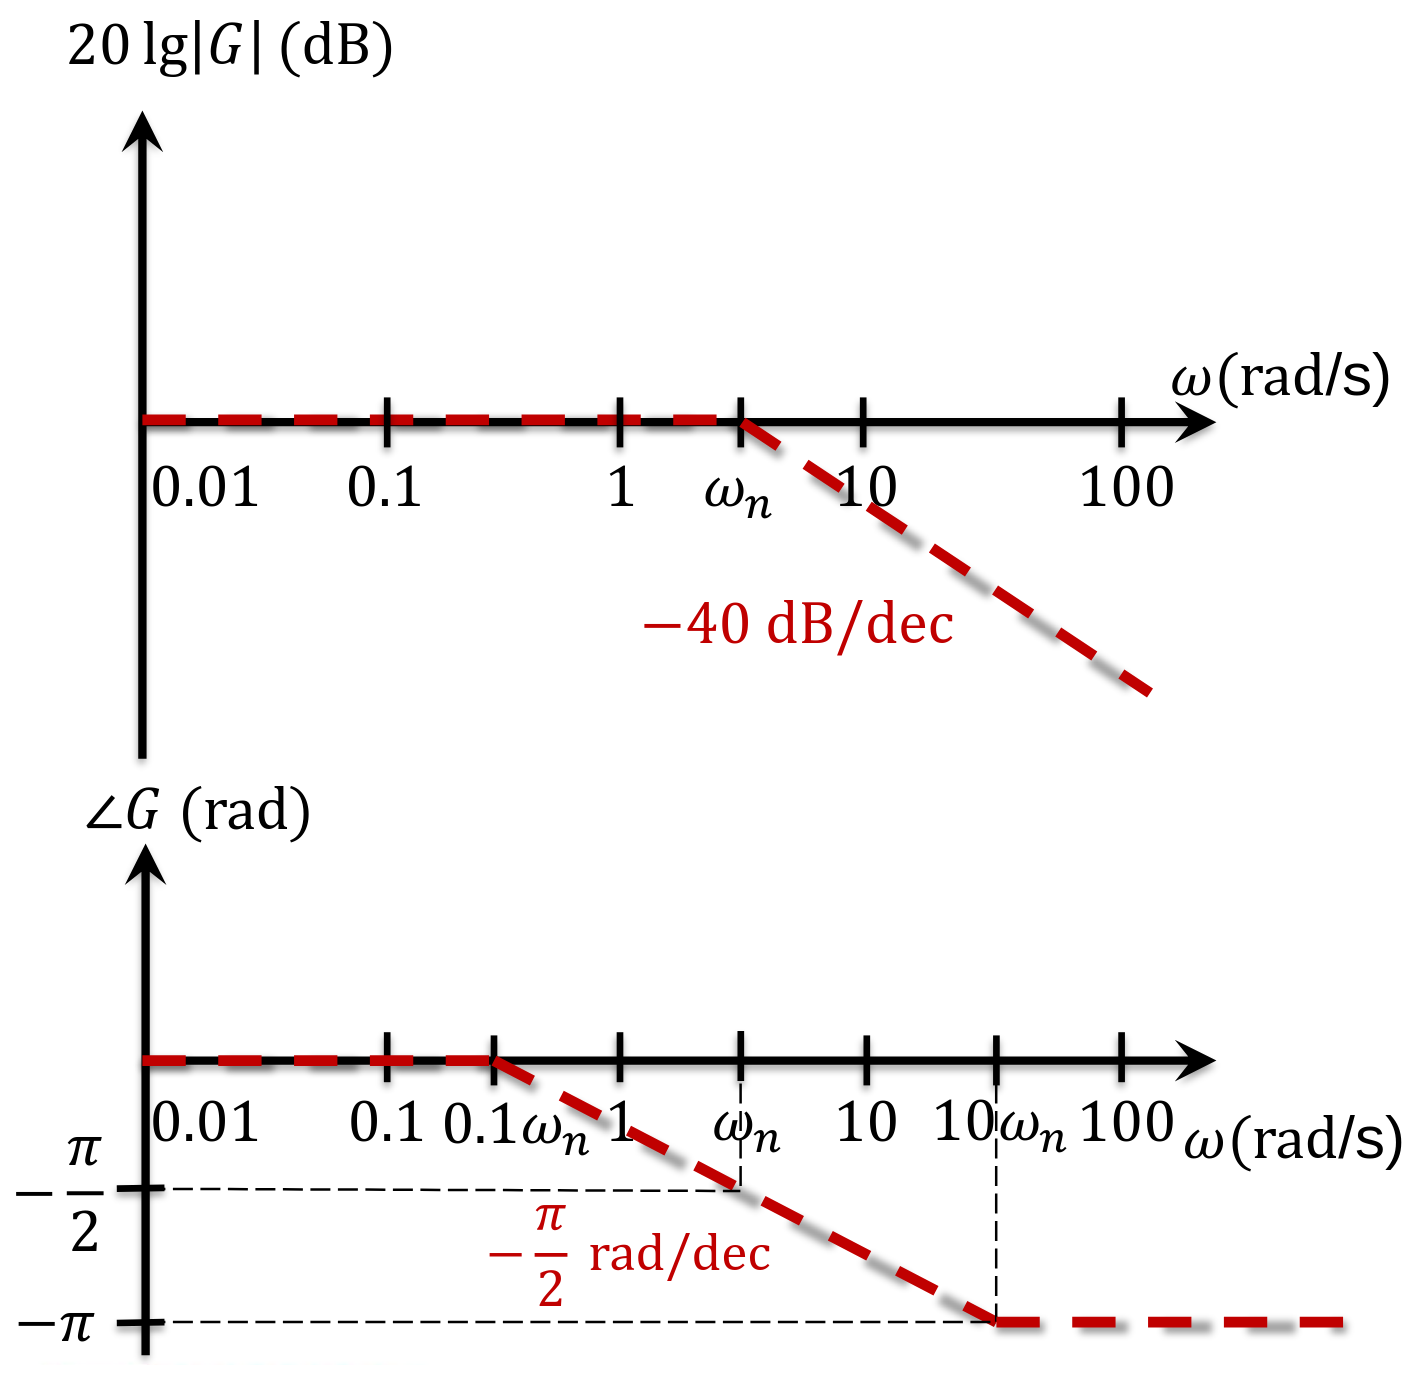
\includegraphics[width=\linewidth]{bode-plots-second-order-pole-plots-2.png}

  Second order zero \(\left(G(s) = \frac{s^2 + 2 \zeta_n s + \omega_n^2}{\omega_n^2}\right)\): \\
  When \(\omega << \omega_n\): \(G(s = j \omega) = 1e^{j0}\) \\
  When \(\omega >> \omega_n\): \(G(s = j \omega) = \frac{\omega^2}{\omega_n^2} e^{j \pi}\) \\
  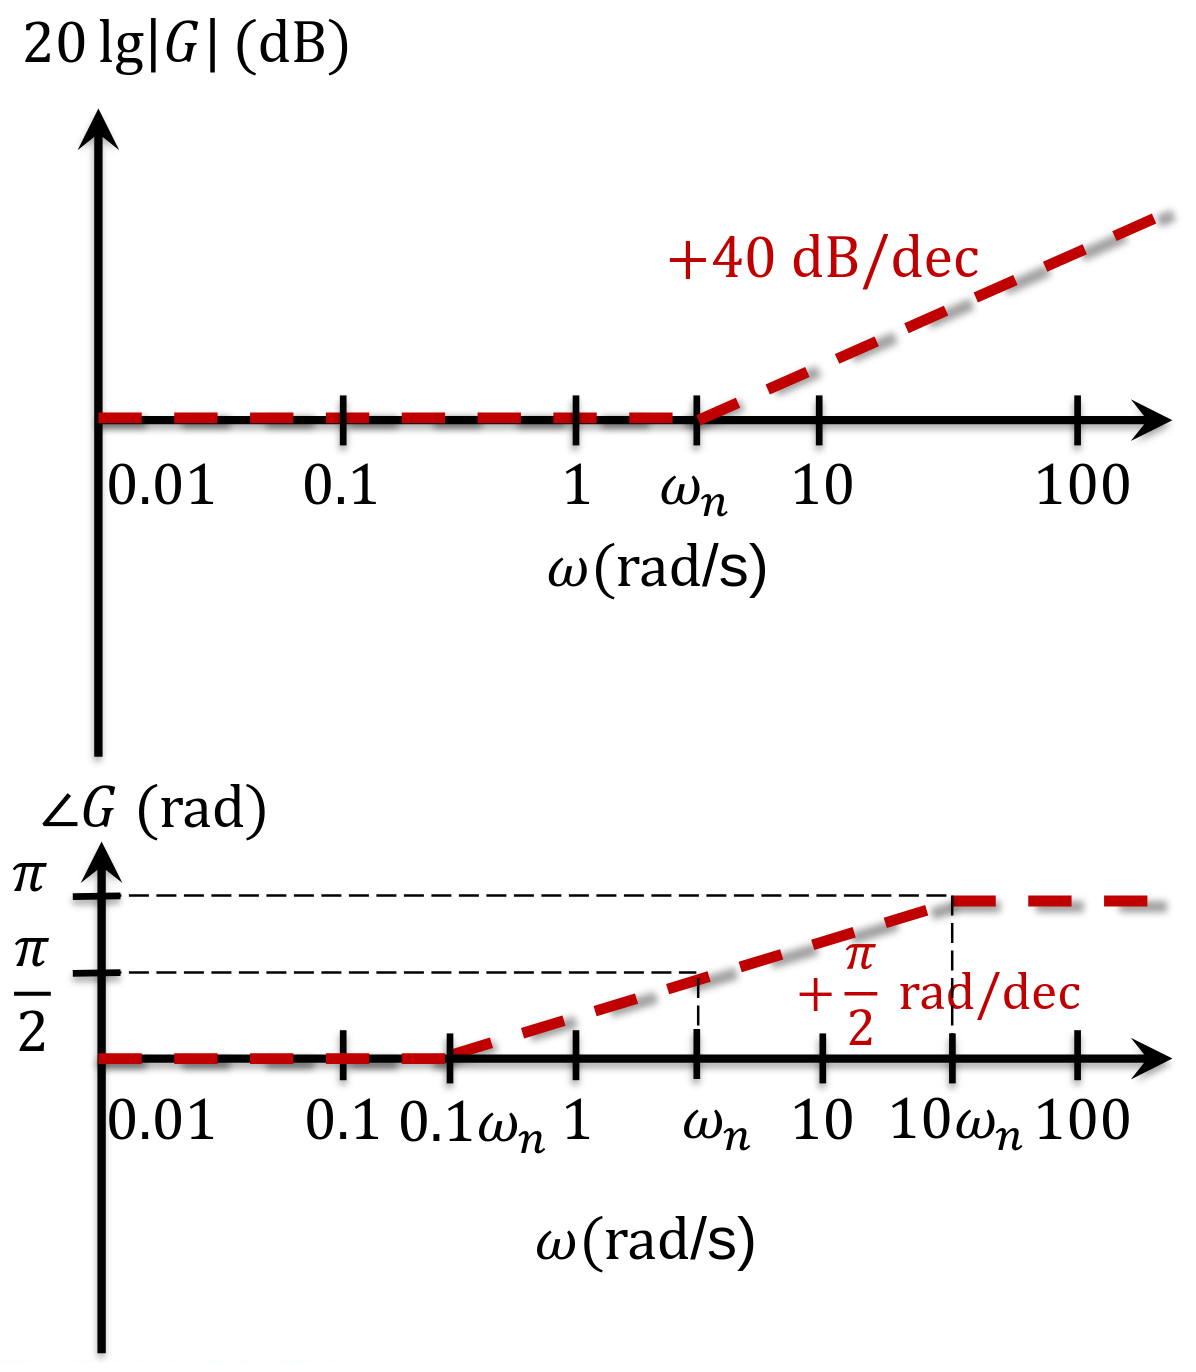
\includegraphics[width=\linewidth]{bode-plots-second-order-zero-plots-2.png}

  \section{Bode plot analysis}

  Low-pass filter: \\
  \(H(s) = \frac{K}{s^2 + bs + a}\)

  Band-pass filter: \\
  \(H(s) = \frac{Ks}{s^2 + bs + a}\)

  High-pass filter: \\
  \(H(s) = \frac{Ks^2}{s^2 + bs + a}\)

  Resonance, \(\zeta < \frac{1}{\sqrt{2}}\): \\
  \(\omega_r = \omega_n \sqrt{1 - 2 \zeta^2}\)

  Gain margin at \(\angle G = \pi\): \\
  \(GM = 0 - \left| G(s = j \omega_{GM}) \right|_{\unit{dB}}\)

  Phase margin at \(|G| = \qty{0}{dB}\): \\
  \(\gamma = \angle G(s = j \omega_{\gamma} + \pi)\)

  Unity feedback is only stable if: \\
  \(\gamma > 0 \text{ and } GM > 0\)

  Closed-loop damping ratio (\(\zeta_{cl}\)): \\
  \(\gamma \uparrow \text{ implies } \zeta_{cl} \uparrow\)

  \subsection{Steady state errors}
  System type 0: \(e_{ss} = \frac{1}{1 + K_p}\) \\
  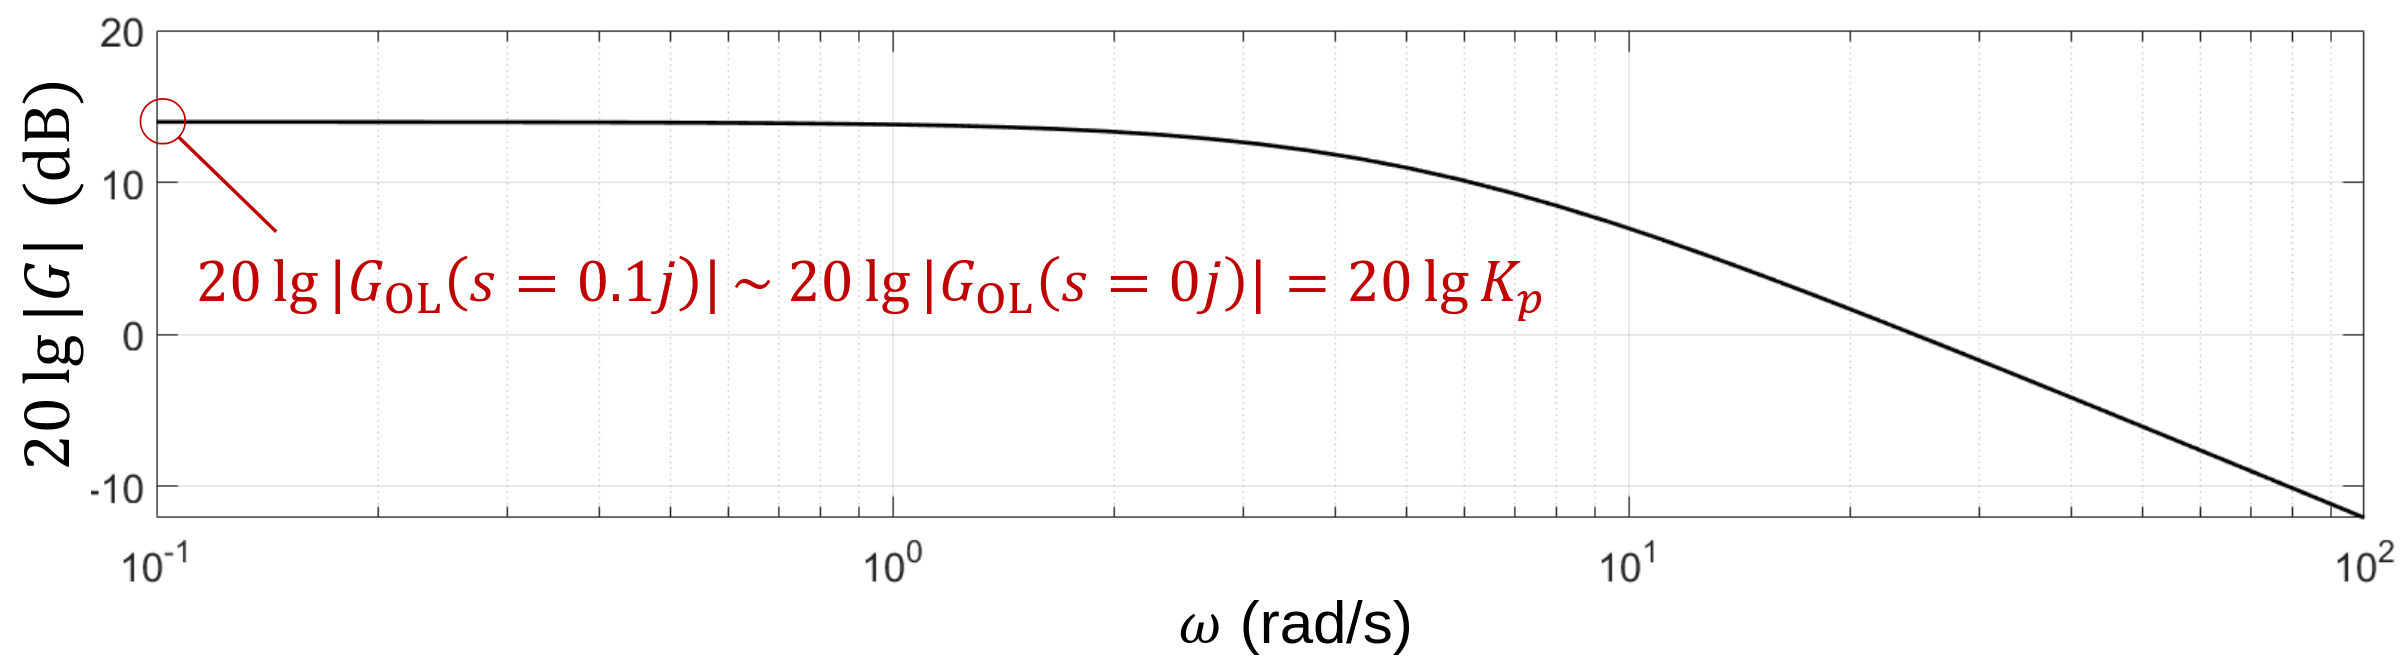
\includegraphics[width=\linewidth]{bode-plots-steady-state-errors-type-0.png}

  System type 1: \(e_{ss} = \frac{1}{K_v}\) \\
  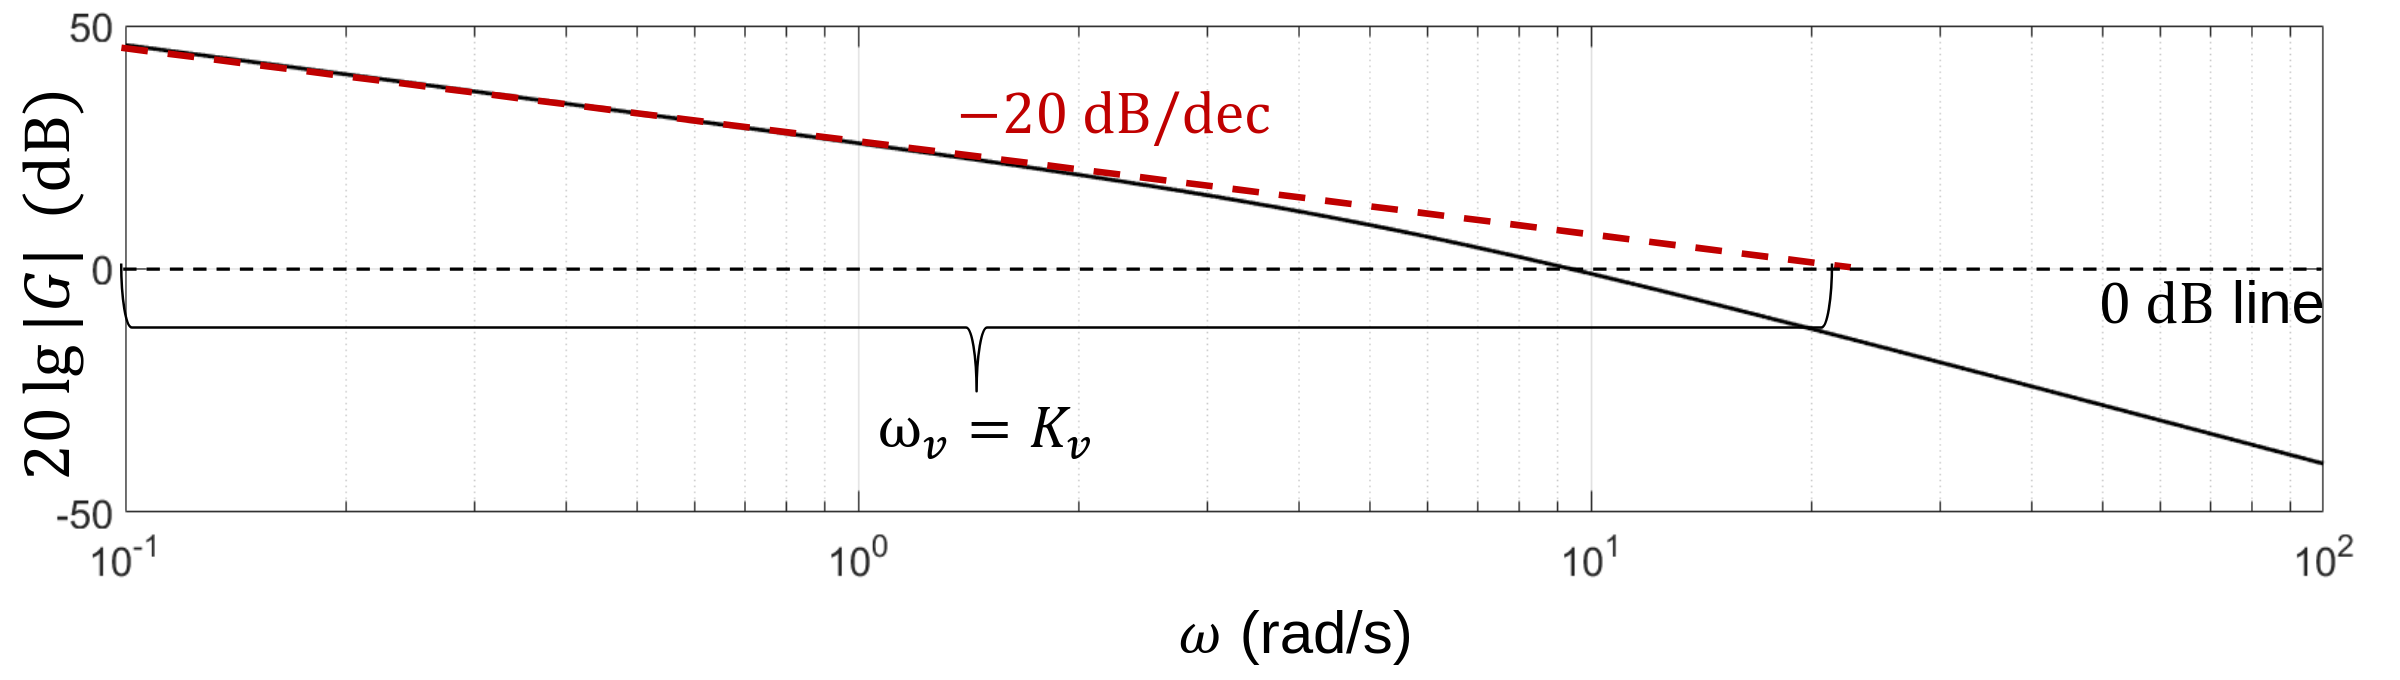
\includegraphics[width=\linewidth]{bode-plots-steady-state-errors-type-1.png}

  \vspace{3em}

  System type 2: \(e_{ss} = \frac{1}{K_a}\) \\
  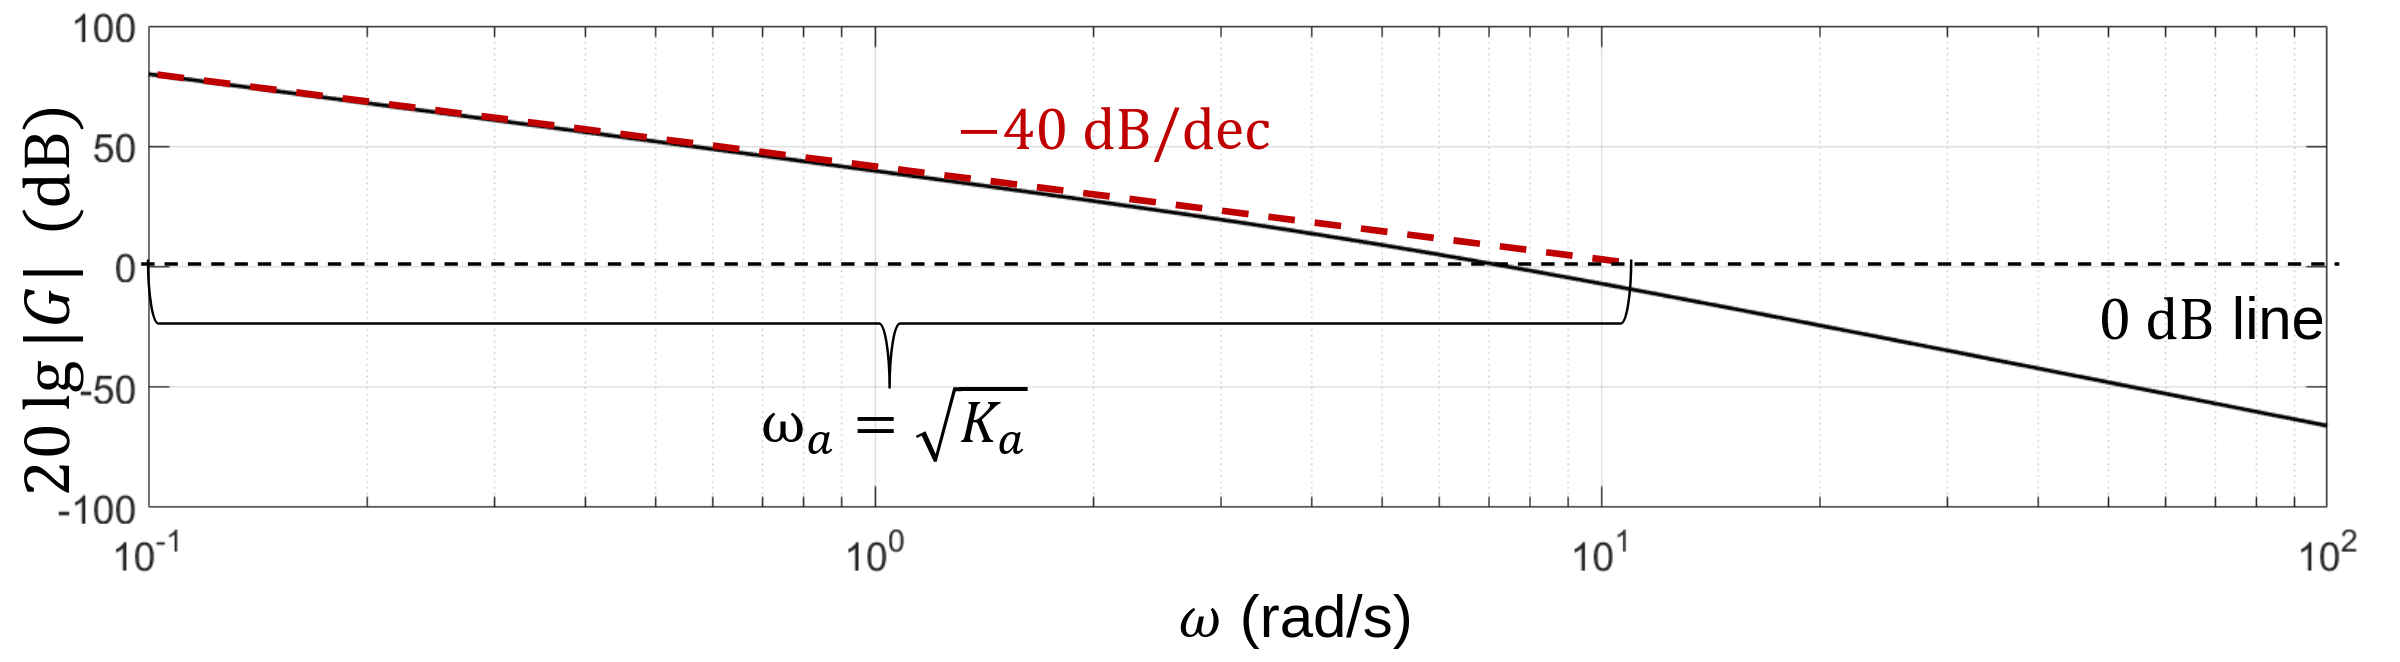
\includegraphics[width=\linewidth]{bode-plots-steady-state-errors-type-2.png}

  \subsection{Steady-steady output of complex functions}
  \(\Diamond\) Set the frequency to the \(\omega\) of the given input function. \\
  \(\Diamond\) Draw a vertical line from the phase graph to the magnitude graph. \\
  \(\Diamond\) Get the phase and magnitude from the graph.

  \subsection{Transfer function approximation (magnitude plot)}
  \(\Diamond\) Check, in the low frequency region, for slopes of \(20n\) and \(-20n\) for \(n\) number of differentiators and integrators respectively. \\
  \(\Diamond\) Search for peaks for second order poles and zeros, and find the frequencies where the slopes start to change, those frequencies will be the corner frequencies. \\
  \(\Diamond\) Sharp peaks can be considered the natural frequency, while gentler ones require using \(\omega_R = \omega_n \sqrt{1 - 2 \zeta^2}\) with the estimated damping ratio to find the natural frequency. Low damping ratio is \(\zeta < 0.1\). \\
  \(\Diamond\) Read the magnitude at the lowest frequency (\(\omega_{low}\)). \\
  \(\Diamond\) If there is no slope, the DC gain is the value, and substitute \(s = 0\) into the transfer function to solve for \(K\). \\
  \(\Diamond\) Otherwise, use that value and substitute \(s = j \omega_{low}\) instead.




  \section{Maths}

  \subsection{Approximation}

  \(1 + \text{Small Value} = 1\) \\
  \(1 + \text{Big Value} = \text{Big Value}\)

  \subsection{Laplace transforms}

  \(\mathcal{L} \left\{k \right\} = \frac{k}{s}, \text{ where } k \text{ is a constant}\) \\
  \(\mathcal{L} \left\{t \right\} = \frac{1}{s^2}\) \\
  \(\mathcal{L} \left\{at \right\} = \frac{a}{s^2}\) \\
  \(\mathcal{L} \left\{\frac{at^n}{n!} \right\} = \frac{a}{s^{n+1}}\) \\
  \(\mathcal{L} \left\{e^{-at} \right\} = \frac{1}{s + a}\) \\
  \(\mathcal{L} \left\{te^{-at} \right\} = \frac{1}{(s + a)^2}\) \\
  \(\mathcal{L} \left\{\frac{1}{(n - 1)!} t^{n - 1}e^{-at} \right\} = \frac{1}{(s + a)^n}\) \\
  \(\mathcal{L} \left\{\sin \omega t \right\} = \frac{\omega}{s^2 + \omega^2}\) \\
  \(\mathcal{L} \left\{\cos \omega t \right\} = \frac{s}{s^2 + \omega^2}\) \\
  \(\mathcal{L} \left\{t \sin \omega t \right\} = \frac{2 \omega s}{(s^2 + \omega^2)^2}\) \\
  \(\mathcal{L} \left\{t \cos \omega t \right\} = \frac{s^2 - \omega^2}{(s^2 + \omega^2)^2}\) \\
  \(\mathcal{L} \left\{e^{-at} \sin \omega t \right\} = \frac{\omega}{(s + a)^2 + \omega^2}\) \\
  \(\mathcal{L} \left\{e^{-at} \cos \omega t \right\} = \frac{s + a}{(s + a)^2 + \omega^2}\) \\
  \(\mathcal{L} \left\{1 - e^{-at} \right\} = \frac{a}{s(s + a)}\) \\
  \(\mathcal{L} \left\{t - \frac{1 -e^{-at}}{a} \right\} = \frac{a}{s^2(s + a)}\) \\
  \(\mathcal{L} \left\{e^{-at} - e^{-bt} \right\} = \frac{b - a}{(s + a) (s + b)}\) \\
  \(\mathcal{L} \left\{be^{-bt} - ae^{-at} \right\} = \frac{(b - a)s}{(s + a) (s + b)}\) \\
  \(\mathcal{L} \left\{(1 - at) e^{-at} \right\} = \frac{s}{(s + a)^2}\) \\
  \(\mathcal{L} \left\{1 - \frac{b}{b - a} e^{- at} + \frac{a}{b - a} e^{-bt} \right\} = \frac{ab}{s (s + a) (s + b)}\) \\
  \(\mathcal{L} \left\{1 - e^{-at} \left(\cos bt + \frac{a}{b} \sin bt \right) \right\} \\ = \frac{a^2 + b^2}{s[(s + a)^2 + b^2]}\) \\
  \(\mathcal{L} \left\{\frac{e^{-at}}{(b - a) (c - a)} + \frac{e^{-bt}}{(c - a) (a - b)} + \frac{e^{-ct}}{(a - c) (b - c)} \right\} \\ = \frac{1}{(s + a) (s + b) (s + c)}\) \\
  \(\mathcal{L} \left\{\frac{\omega}{\sqrt{1 - \zeta^2}} e^{- \zeta \omega t} \sin \omega \sqrt{1 - \zeta^2} t \right\} \\ = \frac{\omega^2}{s^2 + 2 \zeta \omega s + \omega^2}\) \\
  \(\mathcal{L} \left\{1 - \frac{1}{1 - \zeta^2} e^{- \zeta \omega t} \sin \left(\omega \sqrt{1 - \zeta^2} t + \phi \right) \right\} \\ = \frac{\omega^2}{s (s^2 + 2 \zeta \omega s + \omega^2)}, \text{ where } \cos \phi = \zeta\) \\

  \subsection{Derivatives}

  Chain rule: \\
  \(\frac{dz}{dx} = \frac{dz}{dy} \cdot \frac{dy}{dx}\)

  Product rule: \\
  \(\frac{d}{dx} (u \cdot v) = \frac{du}{dx} \cdot v + u \cdot \frac{dv}{dx}\)

  Quotient rule: \\
  \(\frac{d}{dx} \left(\frac{f(x)}{g(x)} \right) = \frac{f'(x) g(x) - f(x) g'(x)}{g(x)^2}\)

  Standard derivatives: \\
  \(\frac{d}{dx} \left(\sin x \right) = \cos x\) \\
  \(\frac{d}{dx} \left(\cos x \right) = - \sin x\) \\
  \(\frac{d}{dx} \left(\arcsin x \right) = \frac{1}{\sqrt{1 - x^2}}\) \\
  \(\frac{d}{dx} \left(\arccos x \right) = - \frac{1}{\sqrt{1 - x^2}}\) \\
  \(\frac{d}{dx} \left(\arctan x \right) = \frac{1}{1 + x^2}\) \\
  \(\frac{d}{dx} \left(\csc x \right) = - \csc x \cot x\) \\
  \(\frac{d}{dx} \left(\sec x \right) = \sec x \tan x\)


  \subsection{Integrals}
  \(\int \sin x \, dx = - \cos x\) \\
  \(\int \cos x \, dx = \sin x\) \\
  \(\int \frac{1}{x^2 + a^2} \, dx = \frac{1}{a} \arctan \left(\frac{x}{a} \right)\) \\
  \(\int \frac{1}{\sqrt{a^2 - x^2}} \, dx = \arcsin \left(\frac{x}{a} \right)\) \\
  \(\int \frac{1}{x^2 - a^2} \, dx = \frac{1}{2a} \ln \left|\frac{x - a}{x + a} \right|\) \\
  \(\int \frac{1}{a^2 - x^2} \, dx = \frac{1}{2a} \ln \left|\frac{a + x}{a - x} \right|\) \\
  \(\int \frac{1}{\sqrt{x^2 - a^2}} \, dx = \ln \left|\sqrt{x^2 - a^2} + x \right|\) \\
  \(\int \tan x \, dx = \ln |\sec x|\) \\
  \(\int \cot x \, dx = \ln |\sin x|\) \\
  \(\int \csc x \, dx = - \ln |\csc x + \cot x|\) \\
  \(\int \sec x \, dx = - \ln |\sec x + \tan x|\)

  Integration by parts: \\
  \(\int u \, dv = uv - \int v \, du\)


  \subsection{Trigonometric identities}

  Quotient identities: \\
  \(\tan \theta = \frac{\sin \theta}{\cos \theta}\) \\
  \(\cot \theta = \frac{\cos \theta}{\sin \theta}\)

  Reciprocal identities: \\
  \(\sin \theta = \frac{1}{\csc \theta}\) \\
  \(\csc \theta = \frac{1}{\sin \theta}\) \\
  \(\cos \theta = \frac{1}{\sec \theta}\) \\
  \(\sec \theta = \frac{1}{\cos \theta}\) \\
  \(\tan \theta = \frac{1}{\cot \theta}\) \\
  \(\cot \theta = \frac{1}{\tan \theta}\)

  Pythagorean identities: \\
  \(\sin^2 \theta + \cos^2 \theta = 1\) \\
  \(\sec^2 \theta - \tan^2 \theta = 1\) \\
  \(\csc^2 \theta - \cot^2 \theta = 1\)

  Even/odd identities: \\
  \(\sin(- \theta) = - \sin \theta\) \\
  \(\cos (- \theta) = \cos \theta\) \\
  \(\tan(- \theta) = - \tan \theta\) \\
  \(\cot (- \theta) = - \cot \theta\) \\
  \(\csc(- \theta) = - \csc \theta\) \\
  \(\sec (- \theta) = \sec \theta\)

  Co-function identities: \\
  \(\sin \left(\frac{\pi}{2} - \theta \right) = \cos \theta\) \\
  \(\cos \left(\frac{\pi}{2} - \theta\right) = \sin \theta \) \\
  \(\tan \left(\frac{\pi}{2} - \theta \right) = \cot \theta\) \\
  \(\cot \left(\frac{\pi}{2} - \theta\right) = \tan \theta \) \\
  \(\csc \left(\frac{\pi}{2} - \theta \right) = \sec \theta\) \\
  \(\sec \left(\frac{\pi}{2} - \theta\right) = \csc \theta \) \\
  \(\frac{\pi}{2} \text{ radians} = 90^{\circ}\)

  Sum/difference identities: \\
  \(\sin (\theta \pm \phi) = \sin \theta \cos \phi \pm \cos \theta \sin \phi\) \\
  \(\cos (\theta \pm \phi) = \cos \theta \cos \phi \mp \sin \theta \sin \phi\) \\
  \(\tan (\theta \pm \phi) = \frac{\tan \theta \pm \tan \phi}{1 \mp \tan \theta \tan \phi}\)

  Double angle identities: \\
  \(\sin (2 \theta) = 2 \sin \theta \cos \theta\) \\
  \(\cos (2 \theta) = \cos^2 \theta - \sin^2 \theta\) \\
  \(\cos (2 \theta) = 2 \cos^2 \theta - 1\) \\
  \(\cos (2 \theta) = 1 - 2 \sin^2 \theta\) \\
  \(\tan (2 \theta) = \frac{2 \tan \theta}{1 - \tan^2 \theta}\)

  Half angle identities: \\
  \(\sin^2 \theta = \frac{1 - \cos (2 \theta)}{2}\) \\
  \(\cos^2 \theta = \frac{1 + \cos (2 \theta)}{2}\) \\
  \(\tan^2 \theta = \frac{1 - \cos (2 \theta)}{1 + \cos (2 \theta)}\)

  % Sum to product of 2 angles: \\
  % \(\sin \theta + \sin \phi = 2 \sin \left( \frac{\theta + \phi}{2} \right) \cos \left( \frac{\theta - \phi}{2} \right)\) \\
  % \(\sin \theta - \sin \phi = 2 \cos \left( \frac{\theta + \phi}{2} \right) \sin \left( \frac{\theta - \phi}{2} \right)\) \\
  % \(\cos \theta + \cos \phi = 2 \cos \left( \frac{\theta + \phi}{2} \right) \cos \left( \frac{\theta - \phi}{2} \right)\) \\
  % \(\cos \theta - \cos \phi = - 2 \sin \left( \frac{\theta + \phi}{2} \right) \sin \left( \frac{\theta - \phi}{2} \right)\)

  % Product to sum of 2 angles: \\
  % \(\sin \theta \sin \phi = \frac{\cos (\theta - \phi) - \cos (\theta + \phi)}{2}\) \\
  % \(\cos \theta \cos \phi = \frac{\cos (\theta - \phi) + \cos (\theta + \phi)}{2}\) \\
  % \(\sin \theta \cos \phi = \frac{\sin (\theta + \phi) + \sin (\theta - \phi)}{2}\) \\
  % \(\cos \theta \sin \phi = \frac{\sin (\theta + \phi) - \sin (\theta - \phi)}{2}\)

  % Law of sines: \\
  % \(\frac{a}{\sin A} = \frac{b}{\sin B} = \frac{c}{\sin C}\)

  % Law of cosines: \\
  % \(a^2 = b^2 + c^2 - 2bc \cos A\)

  % Area of a triangle: \\
  % \(A = \frac{1}{2} ab \sin C\)

\end{multicols*}
\end{document}
